\documentclass[11pt,twoside,a4paper]{article}
\usepackage[margin=2cm]{geometry}
\usepackage{titling}
\usepackage{natbib}
\usepackage{mhchem, textcomp}
\usepackage{chemmacros}
\usepackage[font=small,labelfont=bf]{caption}

\bibliographystyle{model2-names}

\posttitle{\par\end{center}}
\predate{}
\postdate{}
\date{}
\preauthor{\begin{center}}
\postauthor{\par\end{center}\vspace{-0.5em}}
\setlength{\droptitle}{-60pt}

\title{The thermochemical evolution of Mars' deep interior: Geophysical insights with InSight}
\author{Robert Myhill (University of Bristol, UK)}

\begin{document}

\maketitle

NASA's InSight Mission \citep{Banerdtetal2012} is due to land on Mars at the end of 2018. It aims to place new constraints on Mars' formation, evolution and present day internal structure. InSight will determine Mars' thermochemical structure using seismic travel times and waveforms \citep{KOHWDW2006, Teanby2015} recorded by VBB and SP seismometers \citep[the SEIS experiment;][]{Lognonneetal2014}, by using a heat flow probe \citep[HP3;][]{Spohnetal2012} to constrain the thermal gradient in the uppermost lithosphere and by accurately measuring nutations due to the core with an X-band RADAR instrument \citep[RISE;][]{Folkneretal2012}.  These measurements will give us unprecedented constraints on the size and density of the core and on seismic velocities through the planet. 

In order to interpret the data returned from the InSight Mission in terms of internal structure, temperature, chemistry and formation, it is imperative that we have accurate thermodynamic and thermoelastic models of silicates and metallic/sulfidic melts. These models can be used to calculate equilibrium phases and compositions as a function of pressure, temperature and composition. They can also be used to estimate densities and seismic velocities within planetary interiors. The InSight Mission will require such models to interrogate the geophysical data returned from the lander.

\paragraph{Using a combination of lab experiments, thermochemical and seismic modelling, and seismic data interpretation I will add important new inputs to the thermodynamic models used by the planetary community. This additions will enable me to create self-consistent interpretations of Mars' internal thermochemical structure and evolution. My aims will be achieved by the following work packages:}
\begin{enumerate}
\item \textbf{High pressure experiments to determine the role of iron autoredox reactions under conditions appropriate for Mars' interior.} Despite reducing conditions recorded by the SNC meteorites, high pressures are expected to stabilise Fe$^{3+}$ in silicates in the deep interior, precipitating Fe$^0$ as a result. This process fundamentally changes the phase relations in the deep mantle, yet previous works have not yet incorporated these reactions into models of Mars.
\item \textbf{High pressure experiments to isolate the effect of silicate melt composition on high pressure partitioning of trace elements.} One of the primary aims of the InSight Mission is to constrain the chemical composition of Mars' core and conditions of formation. A joint inversion of geophysical data with geochemical data will provide the most accurate information, but existing geochemical models are hindered by a poor understanding of the effect of bulk composition on element partitioning. Improving these models is vital for study of Mars given its uncertain interior chemistry and large-scale heterogeneity. In this work package, I will isolate the effect of silicate melt chemistry on trace element partitioning, thus greatly improving our ability to model core formation and invert data from InSight for the composition of Mars' interior.
\item \textbf{Creation of thermodynamic/thermoelastic models of minerals and melts existing in the deep mantle and core of Mars.} These thermodynamic models are necessary to model seismic velocities in the deep interior as a function of pressure and temperature.
\item \textbf{Geophysical modelling of Mars using InSight data}. The SEIS experiment will be deployed at a single location on Mars surface. At the beginning of the mission, there will be little data, and so this work package will involve the vital task of investigating the effects of a comprehensive range of compositional, thermal and structural parameters on seismic waveforms, and tradeoffs between them. This work will continue to be refined throughout the mission.
\end{enumerate}

These additions to our understanding will be used in conjunction with InSight data to fulfil major mission goals, constraining the thermochemical structure of the deep interior and the formation of the planet over 4.5 billion years ago.

%\subsection*{Work packages}
\subsubsection*{(WP1) The ferric iron content and composition of sulfide in Mars' deep mantle}
\textbf{At pressures exceeding $\sim$6 GPa (600 km in Mars), Fe$^{2+}$ in mantle minerals progressively disproportionates, forming Fe$^{3+}$-bearing silicates \citep[e.g.][]{Frostetal2004, Rohrbachetal2007} in equilibrium with Fe$^0$-bearing metal or sulfide phases. These autoredox reactions fundamentally alter chemical compositions, densities and seismic velocities, and therefore should be included in planetary models, especially when those planets are iron and sulfide-rich (like Mars). However, there is currently little quantitative data on the extent of these reactions as a function of \emph{P}, \emph{T} and chemical composition, without which it is impossible to calculate mineral and melt phase equilibria in Mars' deep interior.  In this work package, I will conduct high pressure laboratory experiments to better quantify the effect of pressure and temperature on the redox state of iron in majoritic garnet under Mars-like conditions. The results will be combined with the few experimental data from the literature to create a thermodynamic solution model for garnets, which can be easily incorporated into software which I will use to calculates densities and seismic velocities as a function of \emph{P}, T and composition in Mars' deep interior.}

Disproportionation of iron in Mars' deep mantle can be described by the following autoredox reaction:
\begin{reaction}
  3 \ce{Fe2SiO4} (ringwoodite) = \ce{Fe3Fe2Si3O12} (garnet) + \ce{Fe} (metal/sulfide)
\end{reaction}
In the Earth, garnet can accommodate over 25\% iron as Fe$^{3+}$ at 14 GPa \citep{Rohrbachetal2007,Rohrbachetal2011}. On Mars, iron contents are much higher than on Earth \citep[Mg\# $\sim$ 75 vs. 90;][]{WD1994}, and the mantle is believed to contain markedly more sulfide \citep[$\sim$6000 vs $<$1000 wt ppm FeS;][]{MS1995,TWW2013}. As a result, autoredox is likely to be at least as important on Mars as on Earth, despite highly reducing conditions at the surface. Because of its major impact on the compositions and properties of both silicate and sulfide phases, it is vitally important to quantify the magnitude of the effect. 

In this study, I will conduct multi-anvil experiments at high pressure with Mars-like mantle compositions in order to determine the effect of \emph{P}, \emph{T} and iron fugacity on Fe$^{3+}$ in garnet. Experiments will be run in a 10/4 assembly (Figure \ref{fig:iron_expts}) at pressures corresponding to Mars' mid-to-lowermost mantle (14, 17 and 20 GPa), and at temperatures of 1600--1900$^{\circ}$C. Iron or metal-metal oxides will be used to buffer the iron and oxygen fugacity of the system via the equilibrium \citep{SOMF2013}:
\begin{reaction}
 2 \ce{Fe2SiO4} + 2 \ce{Mg2SiO4}(ringwoodite) = \ce{Mg4Si4O12} (garnet) + 8 Fe + 4 \ce{O2}
\end{reaction}
Recovered phases will be analysed for ferric iron content with M\"{o}ssbauer spectroscopy. 

\begin{figure}[!ht]
  \centering
  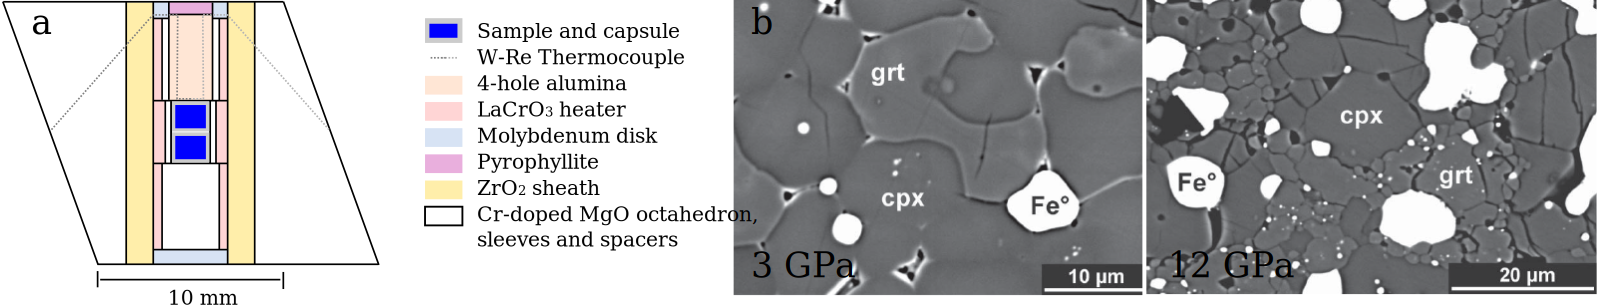
\includegraphics[width=0.95\textwidth]{figures/autoredox}
  \caption{a) Multi-anvil assembly. b) Back-scattered electron images of a recovered charge from multi-anvil runs of \cite{Rohrbachetal2007}, showing precipitation of metallic iron from Fe$^{3+}$-rich garnet at 12 GPa. Models of Mars' deep interior currently include only ferrous iron, and so cannot accurately model compositions at high pressures.}
  \label{fig:iron_expts}
\end{figure}

I will use the results from this work to calculate the amount of ferric iron and composition of sulfide in ultramafic rocks as a function of pressure, temperature and composition. These calculations will be used to create new interior structure models of Mars which can output the speciation of iron within mineral and sulfide phases throughout the mantle, and the resultant densities and seismic velocities. One of the exciting things about this project is that the new geophysical data from InSight will reveal the state of major element (dis)equilibrium between Mars' core and mantle.

\subsubsection*{(WP2) The effect of mantle composition on partitioning of elements during core formation on Mars}

\textbf{The formation of Mars' core was facilitated by large scale melting of the mantle, which allowed large amount of metallic melt to segregate from its silicate host. Slow diffusion in solid silicates suggests that the compositions of the core and mantle have not changed significantly after formation. Therefore, geochemical data on the mantle abundances of siderophile or chalcophile elements (elements which are more compatible in metals and silicates) can be used to decipher the conditions (especially \emph{P}, \emph{T} and \emph{f}O$_2$) of core formation. These conditions also control the amounts of light elements in the core \citep{Rubieetal2015}. Combining these constraints with the geophysical data from InSight thus provides a powerful tool to study the interior of Mars.}

\textbf{Existing experimental data relevant to core formation lack robust constraints on the importance of silicate composition \citep{Righter2016}. Such constraints are vital to modelling efforts, as elements which are sensitive to the conditions of core formation are also highly sensitive to melt composition (i.e. the high valence elements). In this work package, I will equilibrate nominally pure siderophile W, Mo, Nb and Ta with silicate melts at fixed pressure and temperature. These metals are particularly useful for determining the conditions of core formation \citep{OBE2008,CHBBD2014}. The concentrations of these elements will be measured with LA-ICP-MS to quantify the strength of their interactions with the silicate melts. The newly created models for trace element incorporation that can then be used in joint inversions with geophysical data from the InSight Missions \citep[see WP3;][]{BBPSR2015} to constrain the chemical composition of Mars' core and the conditions under which it formed.}

I will initially conduct multi-chamber multi-anvil experiments at 10 GPa and 2200$^{\circ}$C. Capsule materials will be the siderophile metal of interest, preloaded with a small amount of metal oxide to buffer the system. Silicate melt powders of different compositions will be loaded into the capsules. Previous experiments on hydrous melts have shown that pressure is sufficient to close the system when metal foils are used as lids, even in the presence of melt (Myhill et al., 2016). Samples will be heated, held at temperature for long enough to reach equilibrium (this should be <5 minutes, but timescales will be assessed during the experiments) and then quenched. Samples will be recovered and exposed. Major and trace element concentrations in the metals, metal oxides and melts will be measured using EPMA and LA-ICP-MS. Activity coefficients will then be calculated (assuming a certain valence state) using the equilibrium reaction between a metal $M$ and its oxide \ce{MO_{n/2}} (silicate melt) = M (metal) + $\frac{n}{4}$\ce{O2} \{3\}:

\begin{equation}
  \ln \gamma_{MO_{n/2}}  = \frac{\Delta G^{\circ}_{\{3\}}}{RT} - \frac{n}{4} \ln f\textrm{O}_2 + \ln \left( \frac{X_M}{X_{MO_{n/2}}} \right) + \ln \gamma_M
  \label{eqn:mo_eqm}
\end{equation}

The first two terms on the right hand side (functions of the standard state Gibbs energy and oxygen fugacity) are constant at fixed \emph{P} and \emph{T}. The third is the partition function $D(M)$, and the fourth is the log of the activity coefficient of M in the metal phase ($\sim$1). I will re-express the composition-dependent $\gamma_{MO_{n/2}}$ values in terms of interaction parameters (e.g., for a Margules model, $A(\mathbf{x}) = \ln \gamma_{MO_{n/2}} / (1-X_{MO_{n/2}})^2$). Equation \ref{eqn:mo_eqm} can then be used to create accurate models for $\gamma_M$ in iron-rich metallic melts using data from iron-metal/silicate experiments. This technique has three major benefits. Firstly, it circumvents the need to simultaneously fit the complex (and unknown) activity relationships in an Fe-Si-O-C-S metal with similarly complex activity relationship in silicate melts. Secondly, not using the highly reactive MgO capsules common to most partitioning experiments will greatly improve accuracy and reproducability. Finally, this strategy allows me to investigate the effects of varying \emph{P}, \emph{T} and oxygen fugacity on trace element incorporation into silicate melts, which has previously been inaccessible. %It seems likely that common trends between siderophile elements at 1 bar \citep{OBE2008} might persist to higher pressure, which, if confirmed by this study, would greatly reduce the number of free parameters in Mars formation simulations.

I will use the models obtained from these experiments to simulate the growth and composition of Mars' core, fitting the available geochemical data from the SNC meteorites \citep[as previously done for Earth;][]{WW2005}, and the geophysical data on the core and mantle from InSight.

\begin{figure}[!ht]
  \centering
  
\includegraphics[width=0.7\textwidth]{figures/Mo_partitioning}
  \caption{Activity coefficients for MoO$_2$ at 1650$^{\circ}$C, as estimated by a) \cite{WW2013} (based partially on 1 bar data in equilibrium with Mo metal) and b) \cite{RC2011} (based solely on high pressure data with iron alloys, subject to an unconstrained shift $x$). Note the large discrepancies in compositional dependence of $\gamma$, despite the fits using much of the same data.}
  \label{fig:expt_gammas}
\end{figure} 


\subsubsection*{(WP3) Thermodynamic/thermoelastic models of the deep mantle and core of Mars.}

\textbf{Thermodynamic models are a vital requirement of calculating the mineral compositions, density and seismic velocities within Mars as a function of pressure, temperature and composition. Currently, models for high pressure silicates do not include Fe$^{3+}$ (see WP1), and there are no satisfactory thermodynamic models for metallic melts which simultaneously include important elements such as S, Si, O and H. Furthermore, simple models ignore excess properties of solutions, such as bulk moduli, which are likely to play a significant role in determining the properties of metallic solutions \citep{Kom2014,WMSF2015}. In this work package, I will create a model for majoritic garnets incorporating ferric iron (see WP1), and add sulfur and hydrogen to a recently-developed self-consistent thermodynamic model for light element incorporation into metallic melts \citep{MRF2016}. These additions will allow us to take a potential core composition and predict densities and seismic properties, which can then be compared with those obtained from the InSight Mission. They will also be able to predict the position of the liquidus for a given composition, placing bounds on the temperature of Mars' core.}

In creating thermodynamic models it will become possible to self-consistently model chemical equilibrium and seismic velocities. In the case of the majorite model developed from the experimental results of WP1, the changes will allow us to use InSight data to assess the state of equilibrium between Mars' mantle and core. Meanwhile, the new metallic melt model can be interrogated for density and bulk modulus as a function of \emph{P}, \emph{T} and composition, enabling the geophysical data from the RISE and SEIS experiments to be inverted for a core composition. Although it is believed that Mars' core is sulfur-rich \citep{WD1994, KC2008}, it may contain significant amounts of other elements \citep{Stevenson2001}, depending on the conditions during core formation. The melt model will also be used to predict depths of an outer-inner core boundary based on core composition and a core-mantle boundary temperature (see WP4), as it can be used to calculate liquid isentropes and liquidi (in conjunction with models of solid metals).

With accurate and comprehensive thermodynamic models, the new data from InSight will be able to answer questions such as the temperature and composition of Mars' mantle, the composition of its core, its evolution and crystallisation regime \citep{SSWL2007}. Depending on the various trade-offs (see WP4), it may be possible to constrain core size without observing core phases, or crystallisation regime of the core even if seismic data cannot unambiguously resolve an inner core. 

%Excess bulk moduli , but so far there has been no attempt to create such a model. Working with Dan Frost and Dave Rubie, I have built a thermodynamic model for Si and O in metallic melts (Myhill et al., in prep), using modifications to existing solution models that enable excess bulk moduli to change in a physically reasonable manner as a function of pressure and temperature. This work package seeks to extend that model by adding sulfur, using existing experimental data (e.g. Buono and Walker, 2011; Tsuno et al., 2011).


%Products from project:
%Improved garnet thermodynamic model enabling the calculation of chemical properties in Mars' deep mantle
%A preliminary Fe-Si-O-S metallic/sulfidic melt model, created using 1 bar, high pressure static, and shock data.
%Seismic velocities corresponding to the deep mantle and core of Mars, as a function of pressure, temperature and composition.


\subsubsection*{(WP4) Geophysical modelling of Mars and an assessment of parameter trade-offs and uncertainties.}

\textbf{Creating forward models for Mars' interior provides an efficient way to investigate the effects of different variables on geophysical observables, such as seismic travel times or the moment of inertia. There have not currently been any attempts to systematically investigate the trade-offs between different variables. This is particularly true of Mars' thermal structure and composition, partly because of the unknowns addressed in WP1 and 3, and also partly because of choices of free variables and the richness of information contained in synthetic waveforms. In this work package, I will build interior models of Mars spanning the full range of plausible thermochemical structures, and analyse the trade-offs and uncertainties in parameters of interest in terms of InSight observables (e.g. P-S differential times, receiver functions, core properties, surface heat flow).}

Priors for our forward modelling will be the mass, moment of inertia and k2 Love number of Mars, an assumption of chemical equilibrium in the mantle and core and isentropic temperature gradient in the middle of the mantle and within the core. I shall use mineralogical models from the literature \citep[e.g.][]{SLB2011}, enhanced by the results from WP1,3. 

The free parameters will include the Mg number and SiO$_2$ content of the mantle, thickness of the crust, lithosphere and mantle, composition of the core, and thermal structure parameterised as mantle potential temperature, amount of internal heating and Rayleigh number (a measure of convective vigour). This parameterisation \citep[which will follow that described in][]{MJP2005} has the benefit of being physically meaningful, with parameters of geologic interest, whilst automatically including oft-ignored thermal features such as a lower boundary layer. Recently published thermal models include huge variability in thermal properties; two estimates of the thickness of the conductive lid/thermal boundary layer are 125/$\sim$200 km \citep{NF2013} and 400/$\sim$600 km \citep{KC2008}. Such variations change the moment of inertia significantly and will therefore affect apparent best-fit core properties. Seismic data from InSight should therefore provide important constraints on core properties, even if no core phases are observed. 

I will use the forward models which fit the prior constraints (within uncertainties) to create synthetic waveforms (using TauP, SpecFem). I am currently collaborating with Stefanie Hempel (ISAE Toulouse) to set up the required workflow, taking advantages of new software functionality such as the ability to create synthetics for an oblate spheroid. From these, I will identify diagnostic waveform properties and parameter trade-offs. This study will enable rapid interrogation of data when it arrives from InSight. 

\begin{figure}[!ht]
  \centering
  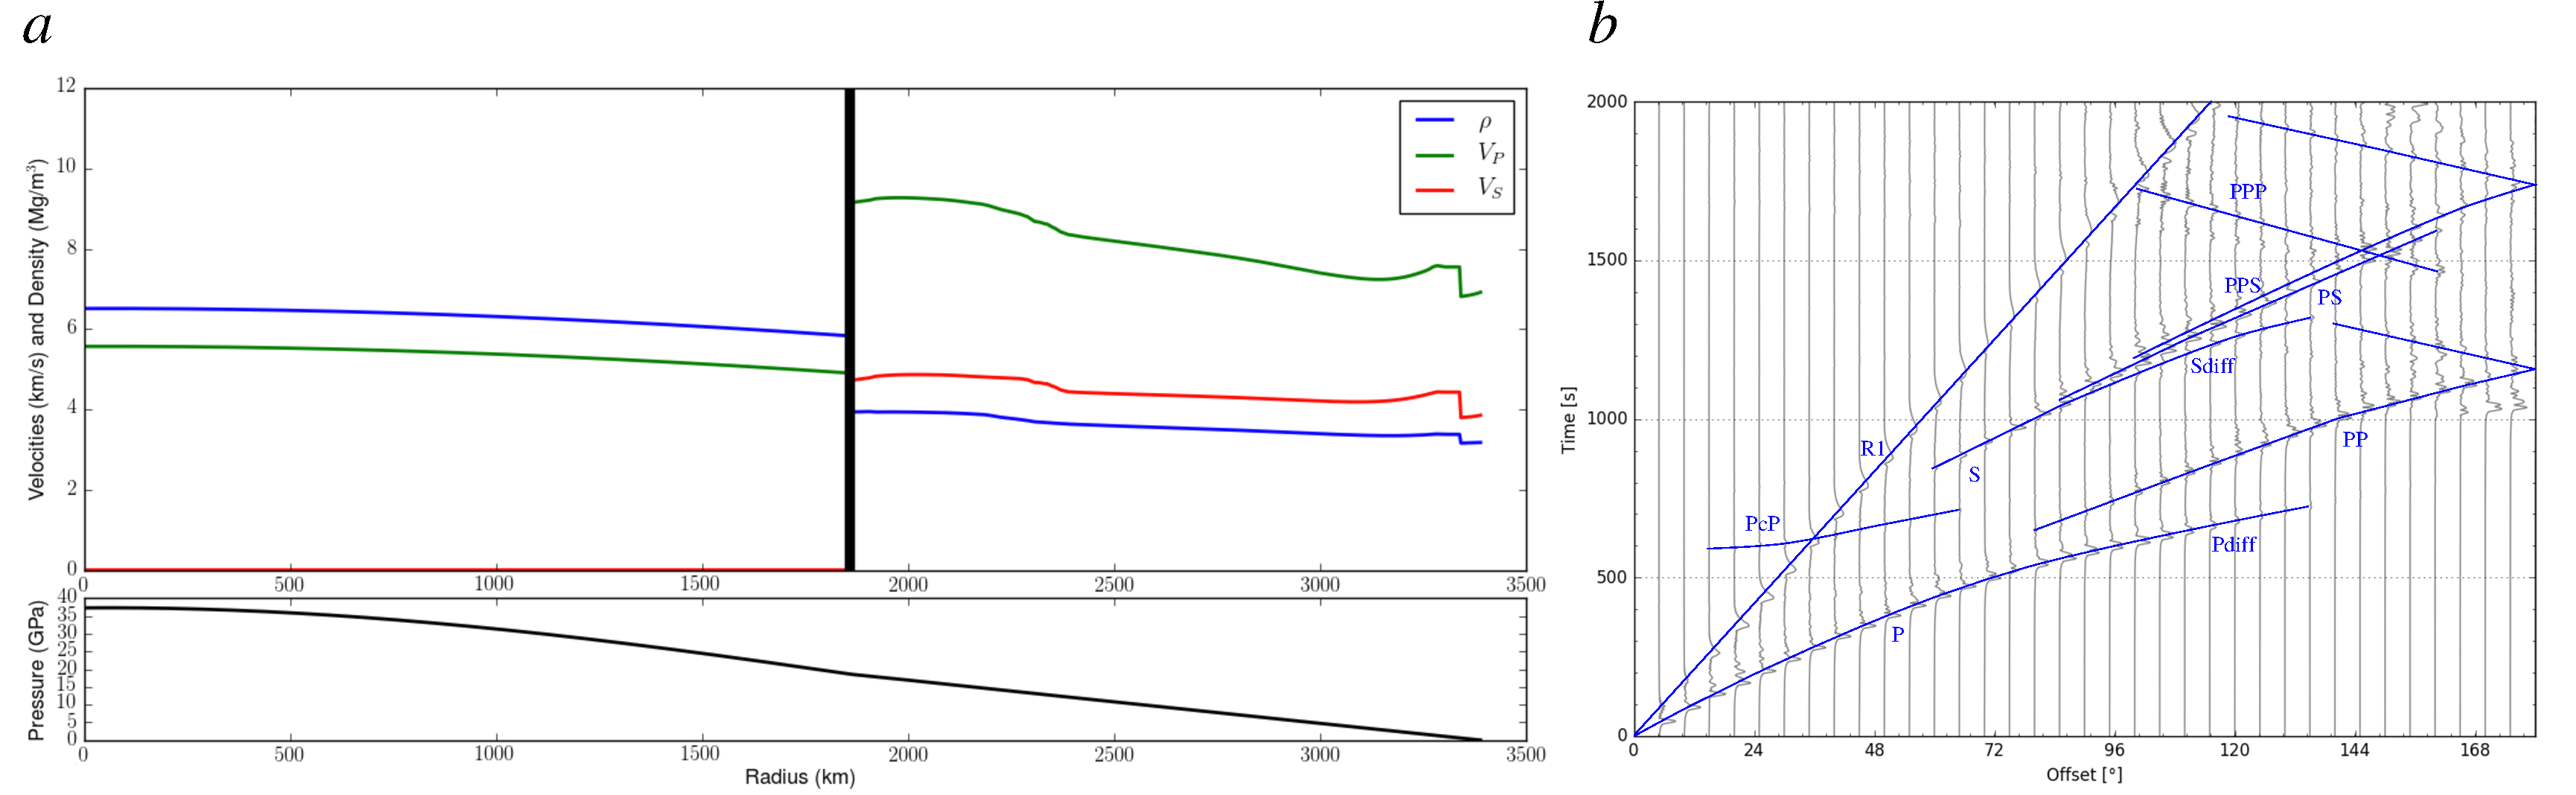
\includegraphics[width=0.95\textwidth]{figures/mars_model}
  \caption{a) Example 1D seismic model of Mars, fitting the mass and moment of inertia of the planet and geochemical estimates of heat-producing elements (U, Th and K). Model includes thermal boundary layers at the top and bottom of the convecting mantle, and a mechanical boundary layer with experimentally-constrained temperature-dependent conductivity. b) Example record section created from a 1D Mars seismic model. Sections like these will be interrogated for seismic arrival times/amplitudes and waveshapes to provide a set of diagnostic tools for the InSight Mission.}
  \label{fig:seismograms}
\end{figure}





\subsection*{Management plan}

Before moving to Bristol, I held a two year Humboldt Fellowship in Germany, designing and running my own projects involving high pressure experiments. I am well-versed in multi-anvil techniques. I have written several papers as a first author with co-authors from different countries. Table \ref{workflow} outlines the expected durations of different part of the project.

\begin{table}[!h]
\centering
\caption{Proposed workflow. E=Experiments, A=Analysis, M=Modelling, W$x$=write-up of paper $x$}
\label{workflow}
\begin{tabular}{l|lll|lll|lll}
  Term starting        & 01/18 & 05/18 & 09/18 & 01/19 & 05/19 & 09/19 & 01/20 & 05/20 & 09/20 \\
  \hline
  WP1 (Majorite)       & E          & A          & W1         & W2         &            &            &            &            &           \\
  WP2 (Partitioning)   &            &            & E          & E          & A          & W3         & A          & W4         &           \\
  WP3 (Modelling)      &            & M          & M/W5       &            &            & M          & W6         &            &           \\
  WP4 (Mars Structure) &            &            &            & A          & A/W?       & A/W?       & A/W?       & A/W?       & A/W?     
\end{tabular}
\end{table}

The University of Bristol conducts annual staff reviews with a senior member of the research staff to ensure research goals are met. It has a comprehensive staff development program, running courses on project management, research leadership. The Faculty finance team provide support for resource management and purchasing.



\subsection*{Relationship to earlier or current work of the applicant/collaborating organisations}

I am currently working on InSight as a PDRA with Nick Teanby and James Wookey on a UKSA grant to study seismometer deployment, regolith properties, and shallow seismic events. On the InSight team I have set up collaborations on synthetic waveform generation with Dr Stefanie Hempel (ISAE Toulouse), which will feed in to WP3 and WP4 of this project. 

I have previous experience on passive seismic techniques, having worked on deep earthquakes for four years as a PhD student at the Bullard Laboratories, University of Cambridge. Following that, I spent three years conducting high pressure experiments at the Bayerisches Geoinstitut as a Humboldt Research Fellow and am well-versed in large and small-volume multi-anvil techniques up to 25 GPa. I have also developed thermodynamic models for high pressure mineral and melt phases in collaboration with Professors Dan Frost and Dave Rubie. I am also one of the developers of the BurnMan project \citep{CHRU2014}, an open-source thermoelastic and thermodynamic toolkit, collaborating with Professor Timo Heister (U.S.A.) and Dr Sanne Cottaar (University of Cambridge).

The proposed research will compliment the existing work at Bristol and in the wider InSight team. There is currently no-one on the InSight team undertaking high pressure experiments or looking at the effects of sulfur and redox state on the questions targeted by the mission. This work will provide a real benefit to many others on the mission, feeding in to larger projects such as the Mars Structural Service, which is aiming to provide near-real-time updates to our best-guess model of Mars' interior.

\subsection*{Justification for resources requested}

\paragraph{Salaried Costs:} I will spend 100\% of my time on the project, the salary is in line with standard UoB banding for a research fellow with 5 years of experience.
\vspace{-1.2em}
\paragraph{Computing Costs (9000 GBP):} The main computing requirement is a desktop that is sufficiently high-specification to create synthetic waveforms from high resolution interior structure models using SpecFEM (5000 GBP). Other costs include a laptop (1000 GBP), data archival hardware (1500 GBP) and other lab and computing consumables (1000 GBP).
\vspace{-1.2em}
\paragraph{Experimental Costs (8640 GBP):} Most multi-anvil experiments will be conducted at the University of Bristol, with some large volume/high pressure runs at the Bayerisches Geoinstitut, Germany. Costs per multianvil experiment ($\sim$200 GBP average over 36 experiments) take into account assembly costs ($\sim$ 50 GBP), cube breakage ($\sim$200 GBP/cube), maintenance and machining, and analysis (LA-ICP-MS, majors via EPMA and ferric iron with M\"{o}ssbauer spectroscopy). Finally, it is expected that there will be some heater failures due to LaCrO$_3$ imperfections. For this reason, total costs are incremented by 20\%.
\vspace{-1.2em}
\paragraph{Travel costs:} During the two years of the mission, there will be quarterly team meetings, but as a relatively junior member of the team, I shall not be required to attend all meetings. Two per year should be sufficient. On top of this, I request funds to present results at one conference per annum - I intend to present results from this project at the LPSC (Texas) and the AGU Fall Meeting (normally in San Francisco). Finally, as I shall be working with researchers in Germany, the States, and France, I request funds for one collaborative visit per annum. 


\clearpage
\bibliography{references}


\end{document}


